\section{Background} \label{back}
\noindent
This section consists of a brief description of the DRAM.



%\begin{figure}[t]
%\centering
%\includegraphics[width=6cm,height=2.5cm]{dram_state.png}
%\caption{Simplified overview of important states of a DRAM}
%\label{fig4}
%\end{figure}

\subsection{Organization of DRAM}\label{b1}
\noindent
Main memory is stored in DRAM cells with higher storage density. DRAM chips are large, rectangular arrays of memory 
cells with support logic for reading, writing data in the arrays and refresh circuitry to maintain the 
integrity of stored data~\cite{wiki:xxx1}. According to storage 
oraganization, memory is hierarchically organized into rank, bank and array. DRAM organization has been 
described in detail in~\cite{Wang:2005:MDM:1104471}.
%Multiple DRAM devices are accessed in parallel 
%which together forms a DRAM rank. DRAM devices in the same rank share the same bus for 
%address and command and another bus for data. For data storage DRAM device is made up of multiple DRAM arrays  
%each of which can be accessed independently. A group of DRAM arrays in different DRAM devices that are 
%accessed together form a DRAM bank. A DRAM bank is a 2D array of cells: rows x columns. 
%Memory arrays are arranged in rows and columns of memory cells called wordlines and bitlines, respectively. Each memory 
%cell has a unique address defined by the intersection of a row and a column. A DRAM cell stores a bit in a 
%capacitor and so they are needed to be charged periodically to prevent data loss. 
Fig.\ref{fig3} shows the organisation of a DRAM.

%\subsection{DRAM access commands}\label{b2}
%\noindent
%DRAM commands such as PRECHARGE, ACTIVATE, READ, WRITE, REFRESH and IDLE are used to 
%access DRAM cells for different DRAM operations. Fig.\ref{fig4} shows a brief overview of the state transition of a DRAM. 
%Transitions in a DRAM can be due to DRAM commands (denoted by curved arrows) or transition triggered by time elapse
%(denoted by straight arrows). 
%Details of the DRAM access commands are given in~\cite{akesson2010introduction}.


%PRECHARGE command precharges the bit lines and a new row is set ready to be accessed. PRECHARGE command is issued before 
%ccessing a new row. After fully precharging the bit lines, the bank goes back to Idle state.
%ACTIVATE command opens a row in a bank for access. The data is transfered from DRAM cells to the row buffer. While in Active 
%state, a READ or a WRITE command may be issued. The same row remains active until a PRECHARGE. 
%READ command initiates a burst read from an active row in a bank.
%WRITE command initiates a burst write to an active row in a bank.
%REFRESH command refreshes the target bank and rows within the DRAM and prevents decaying of data. So it is necessary to 
%issue REFRESH command at regular intervals in order to prevent data loss in DRAMs.

\subsection{Row Buffer Management Policy in DRAM}\label{b3}
\noindent
In DRAM devices, arrays of sense amplifiers act as buffers that provide temporary data storage. Row buffer management policies 
manage the operation of sense amplifiers. In ordinary DRAM devices, two commonly used page policies are-

\begin{itemize}
\item Open-Page policy: The open-page row buffer management policy usually favors memory accesses to the same row of memory by 
keeping the sense amplifiers open and holding the data for ready access. Whenever a row of data is brought to the array of 
sense amplifiers in a DRAM cell, different columns of the same row can be accessed again and again having only column access 
latency. But when a different row of the same bank needs to be accessed, the memory controller first precharges the DRAM 
array, activates the desired row and finally allows for column access. This policy works best for sequential memory accesses 
and performance increases by better exploiting spatial and temporal locality in memory.

\item Close-Page policy: The close-page row buffer management policy works better when we have random memory accesses across
different rows. This policy precharges the row after every memory access. So the bank is in Idle state after every 
row access avoiding the precharging overhead.  
\end{itemize}

The state-of-the-art DRAM controllers mainly use open-page policy. As a result, some real time tasks get prioritised
over other tasks in the waiting queue which may even lead to deadline miss of some of the real time tasks. In the next section, this 
problem has been addressed with the help of a motivating example.

%\subsection{Different timing constraints between DRAM commands}\label{b4}
%\noindent
%Minimum delay must be maintained between two successive DRAM commands to ensure correct operation of a DRAM. Two types of 
%timing constraints exist in DRAM all of which have been accounted in our implementation: 

%\begin{itemize}
%\item Intra Bank Timing constraints- When two successive commands access the same bank, some amount of delay must be 
%maintained. Some intra bank timing constraints include the Row Precharge time, Row Access time, Row to Column delay, 
%Column Access delay and Row Cycle time.

%\begin{itemize}
%\item Row Precharge time- time to precharge a complete row. It is actually the minimum delay between a PRECHARGE command and a subsequent command in the same bank.
%\item Row Access time- minimum time interval between ACTIVATE and onset of next PRECHARGE command in the same bank.
%\item Row to Column delay- time interval between ACTIVATE and a subsequent READ or WRITE command in the same bank.
%\item Column Access delay- time required to access the columns of a particular row in the row buffer.
%\item Row Cycle time- minimum interval to access different rows in the same bank in memory.
%\end{itemize}
%\item Inter Bank Timing constraints- DRAM arrays of different banks are in the same DRAM device. Thus, hardware resources are 
%sharable between banks. Address, commands and even data buses are shared by the ranks. Hence, timing constraints are 
%to be satisfied to avoid conflicts in hardware resources. Some inter-bank timing constraints include the Row activation to Row 
%activation delay and the Data Burst duration.
%\begin{itemize}
%\item Row activation to Row activation delay- time interval between two ACTIVATEs to different banks.
%\item Data Burst duration- busy period of the data bus.
%\end{itemize}
%\end{itemize}



\begin{figure}[t]
\centering
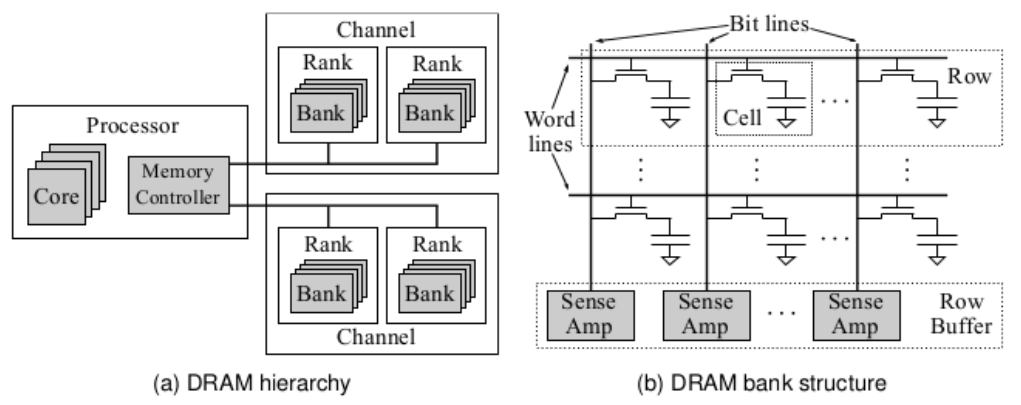
\includegraphics[width=8cm,height=3cm]{Dram_org.png}
\caption{Organisation of DRAM}
\label{fig3}
\end{figure}